% move all configuration stuff into includes file so we can focus on the content
\documentclass[aspectratio=169,hyperref={pdfpagelabels=false,colorlinks=true,linkcolor=white,urlcolor=blue},t]{beamer}

%%%%%%%%%%%%%%%%%%%%%%%%%%%%%%%%%%%%%%%%%%%%%%%%%%%%%%%%%%%%%%%%%%%%%%%%%%%%%%%%%%
%%%%%%%%%%%%%%%%%%%%%%%%%%%%%%%%%%%%%%%%%%%%%%%%%%%%%%%%%%%%%%%%%%%%%%%%%%%%%%%%%%
% packages
\usepackage{pict2e}
\usepackage{epic}
\usepackage{amsmath,amsfonts,amssymb}
\usepackage{units}
\usepackage{fancybox}
\usepackage[absolute,overlay]{textpos} 
\usepackage{media9} % avi2flv: "C:\Program Files\ffmpeg\bin\ffmpeg.exe" -i TuneFreqFilterbank.avi -b 600k -s 441x324 -r 15 -acodec copy TuneFreqFilterbank.flv
\usepackage{animate}
\usepackage{gensymb}
\usepackage{multirow}
\usepackage{silence}
\usepackage[backend=bibtex,style=ieee]{biblatex}
\AtEveryCitekey{\iffootnote{\tiny}{}}
\addbibresource{references}

%%%%%%%%%%%%%%%%%%%%%%%%%%%%%%%%%%%%%%%%%%%%%%%%%%%%%%%%%%%%%%%%%%%%%%%%%%%%%%%%%%
%%%%%%%%%%%%%%%%%%%%%%%%%%%%%%%%%%%%%%%%%%%%%%%%%%%%%%%%%%%%%%%%%%%%%%%%%%%%%%%%%%
% relative paths
\graphicspath{{graph/}}


%%%%%%%%%%%%%%%%%%%%%%%%%%%%%%%%%%%%%%%%%%%%%%%%%%%%%%%%%%%%%%%%%%%%%%%%%%%%%%%%%%
%%%%%%%%%%%%%%%%%%%%%%%%%%%%%%%%%%%%%%%%%%%%%%%%%%%%%%%%%%%%%%%%%%%%%%%%%%%%%%%%%%
% units
\setlength{\unitlength}{1mm}

%%%%%%%%%%%%%%%%%%%%%%%%%%%%%%%%%%%%%%%%%%%%%%%%%%%%%%%%%%%%%%%%%%%%%%%%%%%%%%%%%%
%%%%%%%%%%%%%%%%%%%%%%%%%%%%%%%%%%%%%%%%%%%%%%%%%%%%%%%%%%%%%%%%%%%%%%%%%%%%%%%%%%
% theme & layout
\usetheme{Frankfurt}
\beamertemplatenavigationsymbolsempty
%\setbeamertemplate{frametitle}[smoothbars theme]
\setbeamertemplate{frametitle}
{
    \begin{beamercolorbox}[ht=1.8em,wd=\paperwidth]{frametitle}
        \vspace{-.1em}%
        \hspace{.2em}{\strut\insertframetitle\strut}
        
        \hspace{.2em}\small\strut\insertframesubtitle\strut
        %\hfill
        %
\includegraphics[height=.8cm,keepaspectratio]{CenterMusicTechnology-solid-2lines-white-CoAtag}
        
    \end{beamercolorbox}
    \begin{textblock*}{100mm}(11.6cm,.7cm)
        \includegraphics[height=.8cm,keepaspectratio]{logo_GTCMT_black}
    \end{textblock*}
}

% set this to ensure bulletpoints without subsections
\usepackage{remreset}
\makeatletter
\@removefromreset{subsection}{section}
\makeatother
\setcounter{subsection}{1}

%---------------------------------------------------------------------------------
% appearance
\setbeamercolor{structure}{fg=gtgold}
\setbeamercovered{transparent} %invisible
\setbeamercolor{bibliography entry author}{fg=black}
\setbeamercolor*{bibliography entry title}{fg=black}
\setbeamercolor*{bibliography entry note}{fg=black}

%\usepackage{pgfpages}
%\setbeameroption{show notes}
%\setbeameroption{show notes on second screen=right}
%---------------------------------------------------------------------------------
% fontsize
\let\Tiny=\tiny

%%%%%%%%%%%%%%%%%%%%%%%%%%%%%%%%%%%%%%%%%%%%%%%%%%%%%%%%%%%%%%%%%%%%%%%%%%%%%%%%%%
%%%%%%%%%%%%%%%%%%%%%%%%%%%%%%%%%%%%%%%%%%%%%%%%%%%%%%%%%%%%%%%%%%%%%%%%%%%%%%%%%%
% warnings
\pdfsuppresswarningpagegroup=1
\WarningFilter{biblatex}{Patching footnotes failed}
\WarningFilter{latexfont}{Font shape}
\WarningFilter{latexfont}{Some font shapes}
\WarningFilter{gensymb}{Not defining}


%%%%%%%%%%%%%%%%%%%%%%%%%%%%%%%%%%%%%%%%%%%%%%%%%%%%%%%%%%%%%%%%%%%%%%%%%%%%%%%%%%
%%%%%%%%%%%%%%%%%%%%%%%%%%%%%%%%%%%%%%%%%%%%%%%%%%%%%%%%%%%%%%%%%%%%%%%%%%%%%%%%%%
% title information
\title[]{Introduction to Audio Content Analysis}   
\author[alexander lerch]{alexander lerch} 
%\institute{~}
%\date[Alexander Lerch]{}
\titlegraphic{\vspace{-16mm}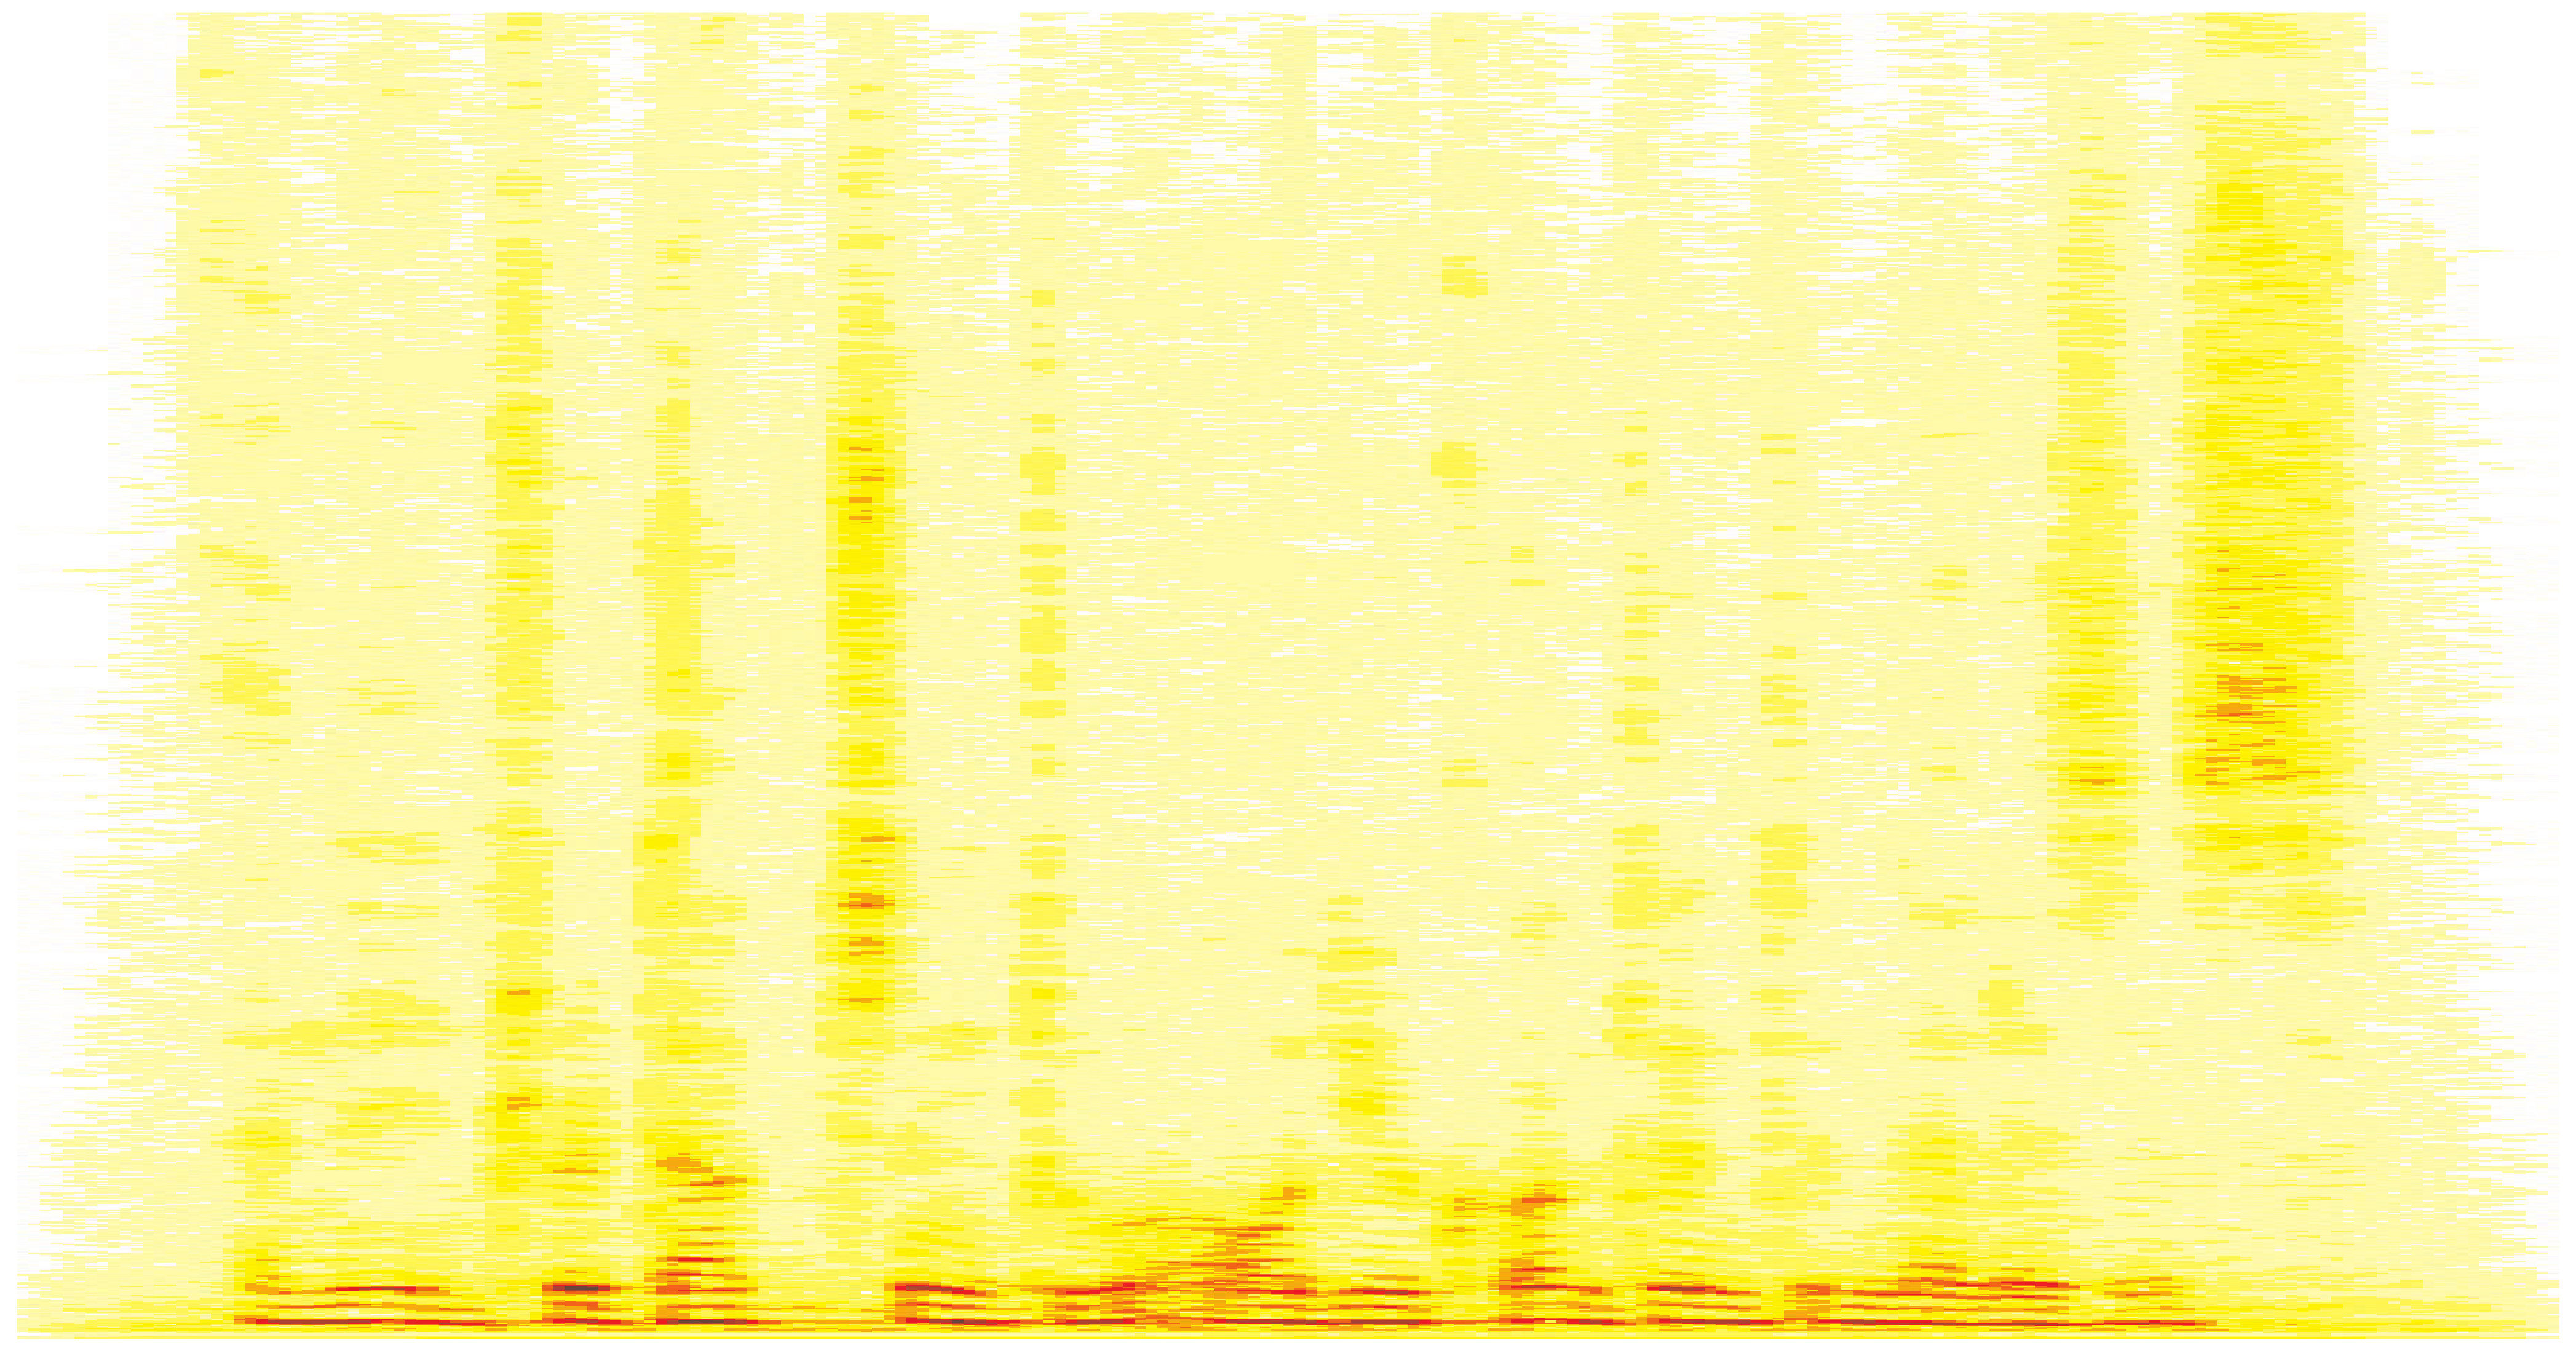
\includegraphics[width=\textwidth,height=3cm]{title}}

%%%%%%%%%%%%%%%%%%%%%%%%%%%%%%%%%%%%%%%%%%%%%%%%%%%%%%%%%%%%%%%%%%%%%%%%%%%%%%%%%%
%%%%%%%%%%%%%%%%%%%%%%%%%%%%%%%%%%%%%%%%%%%%%%%%%%%%%%%%%%%%%%%%%%%%%%%%%%%%%%%%%%
% colors
\definecolor{gtgold}{HTML}{E0AA0F} %{rgb}{0.88,0.66,1,0.06} [234, 170, 0]/256

%%%%%%%%%%%%%%%%%%%%%%%%%%%%%%%%%%%%%%%%%%%%%%%%%%%%%%%%%%%%%%%%%%%%%%%%%%%%%%%%%%
%%%%%%%%%%%%%%%%%%%%%%%%%%%%%%%%%%%%%%%%%%%%%%%%%%%%%%%%%%%%%%%%%%%%%%%%%%%%%%%%%%
% math
\DeclareMathOperator*{\argmax}{argmax}
\DeclareMathOperator*{\argmin}{argmin}
\DeclareMathOperator*{\atan}{atan}
\DeclareMathOperator*{\arcsinh}{arcsinh}
\DeclareMathOperator*{\sign}{sign}
\DeclareMathOperator*{\tcdf}{tcdf}
\DeclareMathOperator*{\si}{sinc}
\DeclareMathOperator*{\princarg}{princarg}
\DeclareMathOperator*{\arccosh}{arccosh}
\DeclareMathOperator*{\hwr}{HWR}
\DeclareMathOperator*{\flip}{flip}
\DeclareMathOperator*{\sinc}{sinc}
\DeclareMathOperator*{\floor}{floor}
\newcommand{\e}{{e}}
\newcommand{\jom}{\mathrm{j}\omega}
\newcommand{\jOm}{\mathrm{j}\Omega}
\newcommand   {\mat}[1]    		{\boldsymbol{\uppercase{#1}}}		%bold
\renewcommand {\vec}[1]    		{\boldsymbol{\lowercase{#1}}}		%bold

%%%%%%%%%%%%%%%%%%%%%%%%%%%%%%%%%%%%%%%%%%%%%%%%%%%%%%%%%%%%%%%%%%%%%%%%%%%%%%%%%%
%%%%%%%%%%%%%%%%%%%%%%%%%%%%%%%%%%%%%%%%%%%%%%%%%%%%%%%%%%%%%%%%%%%%%%%%%%%%%%%%%%
% media9
\newcommand{\includeaudio}[1]{{\includemedia[
                        addresource=audio/#1.mp3,
                        width=5mm,
                        height=5mm,
                        activate=onclick,
                        flashvars={
                            source=audio/#1.mp3  
                            &autoPlay=true
                        }]
                        {
\includegraphics[width=5mm, height=5mm]{SpeakerIcon}}
                        {APlayer.swf}}}
\newcommand{\audioautoplay}[1]{{\begin{center}\includemedia[
                            addresource=audio/#1.mp3,
                            width=.1\linewidth,
                            height=.01\linewidth,
                            activate=pageopen,
                            flashvars={
                                source=audio/#1.mp3  
                                &autoPlay=true
                            }]
                            {}
                            {APlayer.swf}\end{center}}}

\newcommand{\includevideo}[1]{{\begin{center}\includemedia[
                        addresource=video/#1.mp4,
                        width=0.8\linewidth,
                        height=0.4\linewidth,
                        activate=onclick,
                        flashvars={
                            source=video/#1.mp4  
                            &autoPlay=true
                        }]
                        {}
                        {VPlayer.swf}\end{center}}}
\newcommand{\videowithmatlab}[1]{{\begin{center}\includemedia[
                        addresource=video/animate#1.mp4,
                        width=0.8\linewidth,
                        height=0.4\linewidth,
                        activate=onclick,
                        flashvars={
                            source=video/animate#1.mp4  
                            &autoPlay=true
                        }]
                        {}
                        {VPlayer.swf}\end{center}\addreference{matlab source: matlab/animate#1.m}}}
                        

%%%%%%%%%%%%%%%%%%%%%%%%%%%%%%%%%%%%%%%%%%%%%%%%%%%%%%%%%%%%%%%%%%%%%%%%%%%%%%%%%%
%%%%%%%%%%%%%%%%%%%%%%%%%%%%%%%%%%%%%%%%%%%%%%%%%%%%%%%%%%%%%%%%%%%%%%%%%%%%%%%%%%
% other commands
\newcommand{\question}[1]{%\vspace{-4mm}
                          \setbeamercovered{invisible}
                          \begin{columns}[T]
                            \column{.8\textwidth}
                                \textbf{#1}
                            \column{.2\textwidth}
                                \vspace{-8mm}
                                \begin{flushright}
                                     
\includegraphics[scale=.5]{question_mark}
                                \end{flushright}
                                \vspace{6mm}
                          \end{columns}\pause\vspace{-12mm}}

\newcommand{\toremember}[1]{%\vspace{-4mm}
                          \begin{columns}[T]
                            \column{.8\textwidth}
                                \textbf{#1}
                            \column{.2\textwidth}
                                \vspace{-4mm}
                                \begin{flushright}
                                     
\includegraphics[scale=.5]{exclamation_mark}
                                \end{flushright}
                                \vspace{6mm}
                          \end{columns}\vspace{-6mm}}

\newcommand{\matlabexercise}[1]{%\vspace{-4mm}
                          \setbeamercovered{invisible}
                          \begin{columns}[T]
                            \column{.8\textwidth}
                                \textbf{matlab exercise}: #1
                            \column{.2\textwidth}
                                \begin{flushright}
                                     
\includegraphics[scale=.5]{logo_matlab}
                                \end{flushright}
                                %\vspace{6mm}
                          \end{columns}}

\newcommand{\addreference}[1]{  
                  
                    \begin{textblock*}{\baselineskip }(1.12\textwidth,.3\textheight) %(1.15\textwidth,.4\textheight)
                        \rotatebox{90}{\tiny {#1}}
                    \end{textblock*}}
                    
\newcommand{\figwithmatlab}[1]{
                    \begin{figure}
                        \centering
                        \includegraphics{#1}
                        %\label{fig:#1}
                    \end{figure}
                    
                    \addreference{matlab source: \href{https://github.com/alexanderlerch/ACA-Slides/blob/master/matlab/display#1.m}{matlab/display#1.m}}}
\newcommand{\figwithref}[2]{
                    \begin{figure}
                        \centering
                        \includegraphics{#1}
                        \label{fig:#1}
                    \end{figure}
                    
                    \addreference{#2}}  
                                    
\newcommand{\inserticon}[1]{

                    \begin{textblock*}{100mm}(14.5cm,7.5cm)
                        \includegraphics[height=.8cm,keepaspectratio]{#1}
                    \end{textblock*}}            

%%%%%%%%%%%%%%%%%%%%%%%%%%%%%%%%%%%%%%%%%%%%%%%%%%%%%%%%%%%%%%%%%%%%%%%%%%%%%%%%%%
%%%%%%%%%%%%%%%%%%%%%%%%%%%%%%%%%%%%%%%%%%%%%%%%%%%%%%%%%%%%%%%%%%%%%%%%%%%%%%%%%%
% counters
\newcounter{i}
\newcounter{j}
\newcounter{iXOffset}
\newcounter{iYOffset}
\newcounter{iXBlockSize}
\newcounter{iYBlockSize}
\newcounter{iYBlockSizeDiv2}
\newcounter{iDistance}


\subtitle{Module 3.4: Feature Extraction~---~Feature Postprocessing}

%%%%%%%%%%%%%%%%%%%%%%%%%%%%%%%%%%%%%%%%%%%%%%%%%%%%%%%%%%%%%%%%%%%%%%%%%%%%
\begin{document}
    % generate title page
	

\begin{frame}
    \titlepage
    %\vspace{-5mm}
    \begin{flushright}
        \href{http://www.gtcmt.gatech.edu}{\includegraphics[height=.8cm,keepaspectratio]{logo_GTCMT_black}}
    \end{flushright}
\end{frame}


    \section[overview]{lecture overview}
        \begin{frame}{introduction}{overview}
            \begin{block}{corresponding textbook section}
                    \href{http://ieeexplore.ieee.org/xpl/articleDetails.jsp?arnumber=6331120}{Chapter 3~---~Instantaneous Features}: pp.~63--66
            \end{block}

            \begin{itemize}
                \item   \textbf{lecture content}
                    \begin{itemize}
                        \item       derived features
                        \item       feature aggregation
                        \item       feature normalization
                    \end{itemize}
                \bigskip
                \item<2->   \textbf{learning objectives}
                    \begin{itemize}
                        \item       discuss the advantages of specific derived features
                        \item       summarize the principles of feature aggregation
                        \item       list two forms of feature normalization and explain their usefulness
                    \end{itemize}
            \end{itemize}
            \inserticon{directions}
        \end{frame}

   \section[intro]{introduction}
        \begin{frame}{feature post-processing}{introduction 1/2}
            \begin{itemize}
                \item   extracting multiple instantaneous features leads to 
                    \begin{itemize}
                        \item[$\rightarrow$]   one feature vector per block, or
                        \item[$\rightarrow$]   one feature matrix per audio file
                    \end{itemize}
            \end{itemize}
            \bigskip
			\begin{eqnarray*}
				\mat{V} &=& \left[\vec{v}(0)\; 			\vec{v}(1)\; 				\ldots\;	\vec{v}(\mathcal{N}-1)\right]  \nonumber\\ 
				&=& 				 
						\left[ 
				  			\begin{array}{cccc} 
							v_0(0)					&	v_0(1) 					&	\ldots	&	v_0(\mathcal{N}-1)\\
							v_1(0)					&	v_1(1) 					&	\ldots	&	v_1(\mathcal{N}-1)\\
							\vdots					&	\vdots 					&	\ddots		&	\vdots	\\
							v_{\mathcal{F}-1}(0)	&	v_{\mathcal{F}-1}(1) 	&	\ldots	&	v_{\mathcal{F}-1}(\mathcal{N}-1)\\
							\end{array}  
						\right] 
			\end{eqnarray*}
            
            \bigskip
            \begin{footnotesize}
                dimensions:  $\mathcal{F}\times \mathcal{N}$ (number of features and number of blocks, resp.)
            \end{footnotesize}
        \end{frame}
        
        \begin{frame}{feature post-processing}{introduction 2/2}
            
            multiple options for feature matrix processing:
            \begin{enumerate}   
                \item   derive additional features
                \item   aggregate existing features (e.g., one feature vector per file)
                \item   ensure similar scale and distribution
            \end{enumerate}
        \end{frame}

    \section[derived]{derived features}
		\begin{frame}{feature post-processing}{examples of derived features}
            \begin{columns}
                \column{.5\linewidth}
                \begin{itemize}
                    \item   \textbf{diff}: use the change in value
                        \begin{equation*}
                            v_{j,\Delta}(n) = v_j(n) - v_j(n-1) 
                        \end{equation*}
                    \smallskip
                    \item<2-> \textbf{smoothed}: remove high frequency content by low-pass filtering
                        \begin{itemize}
                            \item	 (anticausal) single-pole
                                \begin{equation*}
                                    v_{j,\mathrm{LP}}(n) = (1-\alpha)\cdot v_j(n) - \alpha\cdot v_{j,\mathrm{LP}}(n-1) 
                                \end{equation*}
                            \item	moving average
                        \end{itemize}
                \end{itemize}
                
                \column{.5\linewidth}
                \vspace{-10mm}
                \begin{figure}%
                    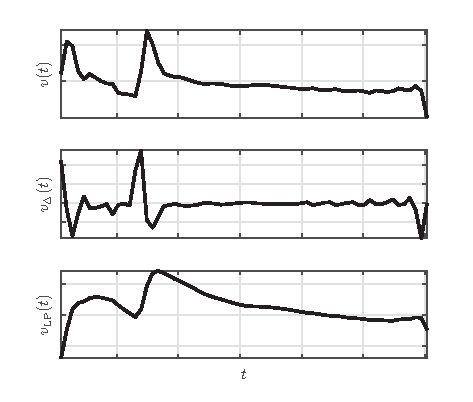
\includegraphics{DerivedFeatures}%
                \end{figure}
            \end{columns}
		\end{frame}

    \section[aggregation]{feature aggregation}
		\begin{frame}{feature post-processing}{feature aggregation}
            feature aggregation:\footnote{also compare \textit{pooling} operation in machine learning} compute \textit{summary features} from feature series $\Rightarrow$ \textbf{subfeatures} 
            
            \bigskip
            \begin{itemize}
                \item \textbf{reasons}
                    \begin{itemize}
                        \item   only one feature vector required per file
                        \item   data reduction
                        \item   characteristics of distribution or change over time contain additional info
                    \end{itemize}
                \smallskip
                \item   \textbf{examples}
                    \begin{itemize}
                        \item   \textit{statistical descriptors}
                            \begin{itemize}
                                \item   mean, median, max, standard deviation
                            \end{itemize}
                                
                        \item   \textit{hand crafted }
                            \begin{itemize}
                                \item anything that might be meaningful --- periodicity, slope, \ldots
                            \end{itemize}
                    \end{itemize}
            \end{itemize}
		\end{frame}

    \section[aggregation]{feature aggregation}
		\begin{frame}{feature post-processing}{feature aggregation}
            \begin{itemize}
                \item       could be for whole file or \textbf{texture window}:\\ split feature series in overlapping blocks of a few seconds length
                \bigskip
                \item<2->   could be \textbf{hierarchical} process:
                    \begin{enumerate}
                        \item   compute subfeatures per window
                        \item   compute subfeatures of subfeature series
                        \item   (go to 1.)
                    \end{enumerate}
            \end{itemize}
		\end{frame}

    \section[normalization]{feature normalization}
		\begin{frame}{feature post-processing}{normalization 1/2}
            \begin{itemize}
                \item   raw features have
                    \begin{itemize}
                        \item	different ranges and scaling factors
                        \item	possibly non-symmetric distributions
                    \end{itemize}
                \smallskip
                \item[$\Rightarrow$]<2->    potential problems with vector distances and some classifiers
                \bigskip
                \item[$\Rightarrow$]<3->    \textbf{feature normalization}
                    \begin{itemize}
                        \item   look at the feature distribution of the whole \textit{training data} set
                        \item   extract statistical descriptors (range, mean, standard deviation)
                        \item   decide for normalization approach
                        \item   normalize both training and test set with \textit{the same} values
                    \end{itemize}
            \end{itemize}
			
		\end{frame}
		\begin{frame}{feature post-processing}{normalization 2/2}
            \begin{itemize}
                \item   \textbf{normalization methods}:
                    \begin{itemize}
                        \item   z-score \[v_{j,\mathrm{N}}(n) = \frac{v_j(n) - \mu_{v_j}}{\sigma_{v_j}}\]
                        \item   range \[v_{j,\mathrm{N}}(n) = \frac{v_j(n) - \min(v_j)}{\max(v_j)-\min(v_j)}\]
                    \end{itemize}
                \item   \textbf{pdf symmetrization}
                    \begin{itemize}
                        \item Box-Cox transform
                            \begin{eqnarray*}
                                v^{(\lambda)} = \left\{ 
                                                \begin{array}{ll} 
                                                    \frac{v^\lambda - 1}{\lambda}, 		& \lambda \neq 0\\ 
                                                    \vphantom{\frac{1}{1}} 	\log(v), 	& \lambda = 0 \\ 
                                                \end{array} 
                                                \right. 
                            \end{eqnarray*}
                        \item   numerical methods \ldots
                    \end{itemize}
            \end{itemize}
             
		\end{frame}
        
    \section{summary}
        \begin{frame}{summary}{lecture content}
            \begin{itemize}
                \item   \textbf{feature matrix should be processed to adapt to task and classifier}
                    \begin{itemize}
                        \item   derive additional features
                        \item   aggregate features
                        \item   normalize features
                    \end{itemize}
                \bigskip
                \item   \textbf{derived features}
                    \begin{itemize}
                        \item   take existing features and ``create'' new ones
                    \end{itemize}
                \bigskip
                \item   \textbf{aggregate features: subfeatures}
                    \begin{itemize}
                        \item   combine blocks of features by computing, e.g., statistical features from them (mean, standard deviation, \ldots)
                        \item   subfeature vector is used as classifier input or as intermediate feature series
                    \end{itemize}
                \bigskip
                \item   \textbf{feature normalization}
                    \begin{itemize}
                        \item   avoid different value ranges might impacting classifier
                        \item   handle different feature distributions
                    \end{itemize}
            \end{itemize}
            \inserticon{summary}
        \end{frame}
\end{document}
